%
% firmware.tex
%
% Copyright (C) 2020 by Universidade Federal de Santa Catarina.
%
% OBDH 2.0 Documentation
%
% This work is licensed under the Creative Commons Attribution-ShareAlike 4.0
% International License. To view a copy of this license,
% visit http://creativecommons.org/licenses/by-sa/4.0/.
%

%
% \brief Firmware chapter.
%
% \author Gabriel Mariano Marcelino <gabriel.mm8@gmail.com>
%
% \institution Universidade Federal de Santa Catarina (UFSC)
%
% \version 0.5.0
%
% \date 2019/10/30
%

\chapter{Firmware} \label{ch:firmware}

\section{Tasks}

A list of the firmware tasks can be seen in the \autoref{tab:firmware-tasks}.

\begin{table}[!h]
    \centering
    \begin{tabular}{lccccc}
        \toprule[1.5pt]
        \textit{Name}          & \textit{Priority} & \textit{Initial delay [ms]} & \textit{Period [ms]} & \textit{Stack [bytes]} \\
        \midrule
        Startup (boot)         & Highest           & 0                           & Aperiodic            & 500                    \\
        Deployment hibernation & Highest           & 0                           & Aperiodic            & TBD                    \\
        Antenna deployment     & Highest           & 0                           & Aperiodic            & TBD                    \\
        Watchdog reset         & Lowest            & 0                           & 100                  & 128                    \\
        Heartbeat              & Lowest            & 0                           & 500                  & 128                    \\
        Beacon                 & Medium            & 1000                        & 60000                & 2000                   \\
        Uplink                 & Low               & 1000                        & 10000                & 500                    \\
        EPS reading            & Medium            & 5000                        & 60000                & TBD                    \\
        EDC reading            & High              & 5000                        & 1000                 & TBD                    \\
        Payload X reading      & Medium            & 5000                        & 5000                 & TBD                    \\
        TTC writing            & Medium            & 5000                        & 10000                & TBD                    \\
        Radio periodoc reset   & Medium            & 600000                      & 600000               & 128                    \\
        System reset           & High              & 0                           & 36000000             & 128                    \\
        Read temperature       & Medium            & 0                           & 60000                & 128                    \\
        CSP Server             & Lowest            & 0                           & 500                  & 1024                   \\
        \bottomrule[1.5pt]
    \end{tabular}
    \caption{Firmware tasks.}
    \label{tab:firmware-tasks}
\end{table}

All these tasks are better described below.

\subsection{Startup (boot)}

.

\subsection{Deployment hibernation}

.

\subsection{Antenna deployment}

.

\subsection{Watchdog reset}

This task resets the internal and external watchdog timer at every 100 ms. The internal watchdog has a maximum count time of 500 ms, and the external watchdog a maximum of 1600 ms (see \autoref{ch:hardware} for more information about the watchdog timers).

To prevent the system to not reset during an anomaly on some task (like an execution time longer than planned), this task has lowest possible priority: 0.

\subsection{Heartbeat}

The heartbeat task keeps blinking a LED (``\textit{System LED}'' in \autoref{fig:status-leds}) at a rate of 1 Hz during the execution of the system. Its purpose is to give a visual feedback of the execution of the scheduler. This is tasks does not have a specific purpose on the flight version of the module (the flight version of the PCB does not have LEDs).

\subsection{Beacon}

.

\subsection{Uplink}

.

\subsection{EPS reading}

.

\subsection{EDC reading}

.

\subsection{Payload X reading}

.

\subsection{TTC writing}

.

\subsection{Radio periodic reset}

.

\subsection{System reset}

This task resets the microcontroller by software at every 10 hours. This can be useful to cleanup possible wrong values in variables, repeat the antenna deployment routine (limited to $n$ times), cleanup the RAM memory, etc.

\subsection{Read temperature}

This task reads the internal temperature of the microcontroller of the OBDH at every 60 seconds.

\subsection{CSP Server}

.

\section{Telemetry}


\subsection{Beacon}

The beacon packet is transmitted at every 1 minute and contains a basic telemetry data of the satellite. The content of this packet can be seen in \autoref{tab:telemetry-beacon}.

\begin{itemize}
    \item Period: 60 seconds
    \item Band: UHF
    \item Condition to operate: Always on
\end{itemize}

\begin{table}[!h]
    \centering
    \begin{tabular}{llc}
        \toprule[1.5pt]
        \textbf{Parameter} & \textbf{Content}       & \textbf{Length [bytes]} \\
        \midrule
        Packet ID          & 10h                    & 1 \\
        Satellite callsign & ``0PY0EGU''            & 7 \\
        $\mu$C temperature & Raw $\mu$C temperature & 2 \\
        $\mu$C voltage     & Raw $\mu$C voltage     & 2 \\
        $\mu$C current     & Raw $\mu$C current     & 2 \\
        Last reset cause   & Last reset cause ID    & 1 \\
        System time        & System time in ticks   & 4 \\
        Radio temperature  & Raw radio temperature  & 4 \\
        Last TC RSSI       & Raw RSSI value         & 2??? \\
        Last received TC   & Last received TC ID    & 1 \\
        Battery 1 voltage  & Raw battery 1 voltage  & 2 \\
        Battery 2 voltage  & Raw battery 2 voltage  & 2 \\
        Battery current    & Raw battery current    & 2 \\
        Battery charge     & Raw battery charge     & 2 \\
        ...                & ...                    & ... \\
        \midrule
        Total              & -                      & 34 \\
        \bottomrule[1.5pt]
    \end{tabular}
    \caption{Beacon packet.}
    \label{tab:telemetry-beacon}
\end{table}

\subsection{EDC Information}

\begin{table}[!h]
    \centering
    \begin{tabular}{llc}
        \toprule[1.5pt]
        \textbf{Parameter} & \textbf{Content}                                 & \textbf{Len. [bytes]} \\
        \midrule
        Packet ID          & 11h                                              & 1 \\
        Satellite callsign & ``0PY0EGU''                                      & 7 \\
        \midrule
        \multicolumn{3}{c}{\textbf{PTT Decoder}} \\
        \midrule
        Time tag           & PTT signal receiving time                        & 4 \\
        Error code         & Error code                                       & 1 \\
        Carrier frequency  & Carrier frequency                                & 2 \\
        Carrier Abs        & Carrier amplitude at ADC interface output        & 2 \\
        Message length     & User message length in bytes                     & 1 \\
        User message       & ARGOS-2 PTT-A2 user message                      & 35 \\
        \midrule
        \multicolumn{3}{c}{\textbf{HK Info}} \\
        \midrule
        Current time       & Current time since J2000 epoch                   & 4 \\
        Elapsed time       & Elapsed time since last reset                    & 4 \\
        Current supply     & System current supply in mA                      & 2 \\
        Voltage supply     & System voltage supply in mV                      & 2 \\
        Temperature        & EDC board temperature                            & 1 \\
        PLL sync bit       & RF front end LO...                               & 1 \\
        ADC RMS            & RMS level at front-end output                    & 2 \\
        Num of RX PTT      & Generated PTT packages since last initialization & 1 \\
        Max                &                                                  & 1 \\
        Memory error count &                                                  & 1 \\
        \midrule
        \multicolumn{3}{c}{\textbf{System State}} \\
        \midrule
        Current time       &                                                  & 4 \\
        PTT available      & Number of PTT Package available for reading      & 1 \\
        PTT is paused      & PTT decoder task status                          & 1 \\
        Sampler state      & ADC sampler state                                & 1 \\
        \midrule
        Total              & -                                                & 79 \\
        \bottomrule[1.5pt]
    \end{tabular}
    \caption{EDC information packet.}
    \label{tab:telemetry-edc}
\end{table}

\subsection{EDC Samples}

The EDC samples are XX bytes long and are transmitted in Y packets with 219 bytes each

\begin{table}[!h]
    \centering
    \begin{tabular}{llc}
        \toprule[1.5pt]
        \textbf{Parameter} & \textbf{Content}               & \textbf{Length [bytes]} \\
        \midrule
        Packet ID          & 12h                            & 1 \\
        Satellite callsign & ``0PY0EGU''                    & 7 \\
        Time tag           & Elapsed time since J2000 epoch & 4 \\
        Packet counter     & ADC sample packet number       & 1 \\
        I sample[n]        & First ADC I-sample             & 2 \\
        Q sample[n]        & First ADC Q-sample             & 2 \\
        ...                & ...                            & ... \\
        I sample[n+102]    & First ADC I-sample             & 2 \\
        Q sample[n+102]    & First ADC Q-sample             & 2 \\
        \midrule
        Total              & -                              & 219 \\
        \bottomrule[1.5pt]
    \end{tabular}
    \caption{EDC samples packet.}
    \label{tab:telemetry-edc-samples}
\end{table}

\section{Telecommands}

\begin{table}[!h]
    \centering
    \begin{tabular}{lll}
        \toprule[1.5pt]
        \textbf{Name}          & \textbf{Parameters}           & \textbf{Access} \\
        \midrule
        Enter hibernation      & Hibernation period in seconds & Private         \\
        Leave hibernation      & None                          & Private         \\
        Activate beacon        & None                          & Private         \\
        Deactivate beacon      & None                          & Private         \\
        Activate downlink      & None                          & Private         \\
        Deactivate downlink    & None                          & Private         \\
        Activate EDC           & None                          & Private         \\
        Deactivate EDC         & None                          & Private         \\
        Get EDC info           & None                          & Private         \\
        Activate Payload X     & Experiment period in seconds  & Private         \\
        Deactivate Payload X   & None                          & Private         \\
        Set system time        & Time value (epoch)            & Private         \\
        Ping                   & None                          & Public          \\
        Message broadcast      & ASCII message                 & Public          \\
        Request data           & Data flags                    & Public          \\
        \bottomrule[1.5pt]
    \end{tabular}
    \caption{System telecomamnds.}
    \label{tab:system-telecommands}
\end{table}

\subsection{Enter hibernation}

\begin{table}[!h]
    \centering
    \begin{tabular}{lll}
        \toprule[1.5pt]
        \textbf{Parameter}      & \textbf{Content}                         & \textbf{Length [bytes]} \\
        \midrule
        Packet ID               & 20h                                      & 1 \\
        Ground station callsign & Any callsign (ASCII, filled with ``0''s) & 7 \\
        Hibernation period      & Period in minutes (1 to 65535)           & 2 \\
        Key                     & Telecommand key (ASCII)                  & 10 \\
        \midrule
        Total                   & -                                        & 20 \\
        \bottomrule[1.5pt]
    \end{tabular}
    \caption{Enter hibernation telecommand.}
    \label{tab:enter-hibernation-tc}
\end{table}

\subsection{Leave hibernation}

\begin{table}[!h]
    \centering
    \begin{tabular}{lll}
        \toprule[1.5pt]
        \textbf{Parameter}      & \textbf{Content}                         & \textbf{Length [bytes]} \\
        \midrule
        Packet ID               & 21h                                      & 1 \\
        Ground station callsign & Any callsign (ASCII, filled with ``0''s) & 7 \\
        Key                     & Telecommand key (ASCII)                  & 10 \\
        \midrule
        Total                   & -                                        & 18 \\
        \bottomrule[1.5pt]
    \end{tabular}
    \caption{Leave hibernation telecommand.}
    \label{tab:leave-hibernation-tc}
\end{table}

\subsection{Activate beacon}

.

\subsection{Deactivate beacon}

.

\subsection{Activate EDC}

.

\subsection{Deactivate EDC}

.

\subsection{Get EDC info}

This telecommand request information from the EDC payload. When received, the OBDH transmits the housekeeping and state frames of the EDC module (28 bytes). This telecommand does not requires a key.

\subsection{Activate Payload X}

.

\subsection{Deactivate Payload X}

.

\subsection{Set system time}

.

\subsection{Ping}

\begin{table}[!h]
    \centering
    \begin{tabular}{lll}
        \toprule[1.5pt]
        \textbf{Parameter}      & \textbf{Content}                         & \textbf{Length [bytes]} \\
        \midrule
        Packet ID               & 22h                                      & 1 \\
        Ground station callsign & Any callsign (ASCII, filled with ``0''s) & 7 \\
        \midrule
        Total                   & -                                        & 8 \\
        \bottomrule[1.5pt]
    \end{tabular}
    \caption{Ping telecommand.}
    \label{tab:ping-tc}
\end{table}

\begin{table}[!h]
    \centering
    \begin{tabular}{lll}
        \toprule[1.5pt]
        \textbf{Parameter}      & \textbf{Content}                               & \textbf{Length [bytes]} \\
        \midrule
        Packet ID               & 12h                                            & 1 \\
        Satellite callsign      & ``PY0EGU''                                     & 7 \\
        Destination callsign    & Requester callsign (ASCII, filled with ``0''s) & 7 \\
        \midrule
        Total                   & -                                              & 15 \\
        \bottomrule[1.5pt]
    \end{tabular}
    \caption{Ping telecommand answer.}
    \label{tab:ping-tc-ans}
\end{table}

\subsection{Message broadcast}

\begin{table}[!h]
    \centering
    \begin{tabular}{lll}
        \toprule[1.5pt]
        \textbf{Parameter}      & \textbf{Content}                         & \textbf{Length [bytes]} \\
        \midrule
        Packet ID               & 23h                                      & 1 \\
        Ground station callsign & Any callsign (ASCII, filled with ``0''s) & 7 \\
        Message                 & Message to broadcast (ASCII)             & up to  \\
        \midrule
        Total                   & -                                        & 8 \\
        \bottomrule[1.5pt]
    \end{tabular}
    \caption{Message broadcast telecommand.}
    \label{tab:msg-broadcast-tc}
\end{table}

\subsection{Request data}

.

\section{Operating System}

As operating system the FreeRTOS 10 \cite{freertos} is being used. FreeRTOS is a market-leading real-time operating system (RTOS) for microcontrollers and small microprocessors. Distributed freely under the MIT open source license, FreeRTOS includes a kernel and a growing set of IoT libraries suitable for use across all industry sectors. FreeRTOS is built with an emphasis on reliability and ease of use.

The main configuration parameters of the operating system in this project are availabe in \autoref{tab:freertos-config}.

\begin{table}[!h]
    \centering
    \begin{tabular}{lrr}
        \toprule[1.5pt]
        \textbf{Parameter}       & \textbf{Value} & \textbf{Unit} \\
        \midrule
        Version                  & v10.2.0        & - \\
        Tick rate (Hz)           & 1000           & Hz \\
        CPU clock (HZ)           & 32             & MHz \\
        Max. priorities          & 5              & - \\
        Heap size                & 40960          & bytes \\
        Max. length of task name & 20             & - \\
        \bottomrule[1.5pt]
    \end{tabular}
    \caption{FreeRTOS main configuration parameters.}
    \label{tab:freertos-config}
\end{table}

More details of the used configuration parameters can be seen in the file \textit{\href{https://github.com/spacelab-ufsc/obdh2/blob/master/firmware/config/FreeRTOSConfig.h}{firmware/config/FreeRTOSConfig.h}} from \cite{obdh2-repo}.

\section{Hardware Abstraction Layer (HAL)}

As the Hardware Abstraction Layer (HAL\nomenclature{\textbf{HAL}}{\textit{Hardware Abstraction Layer.}}), the DriverLib \cite{driverlib} from Texas Instruments is begin used. It is the official API to access the registers of the MSP430 microcontrollers.

The DriverLib is meant to provide a ``software'' layer to the programmer in order to facilitate higher level of programming compared to direct register accesses. By using the high level software APIs provided by DriverLib, users can create powerful and intuitive code which is highly portable between not only devices within the MSP430 platform, but between different families in the MSP430/MSP432 platforms.

\section{File System}

As file system, the Reliance Edge library is used \cite{reliance_edge} (version 2.4). Reliance Edge is a failsafe filesystem with an small footprint, targeting critical embedded systems with fewer resources. It works with a broad array of storage media including: eMMC, SD/MMC, NVRAM, USB mass storage and SATA (or PATA) disk.

\section{Protocols}

\subsection{NGHam}

NGHam \cite{ngham}, short for Next Generation Ham Radio, is a set of protocols for packet radio communication. Its usage is similar to the existing AX.25 protocol.

\begin{figure}[!ht]
    \begin{center}
        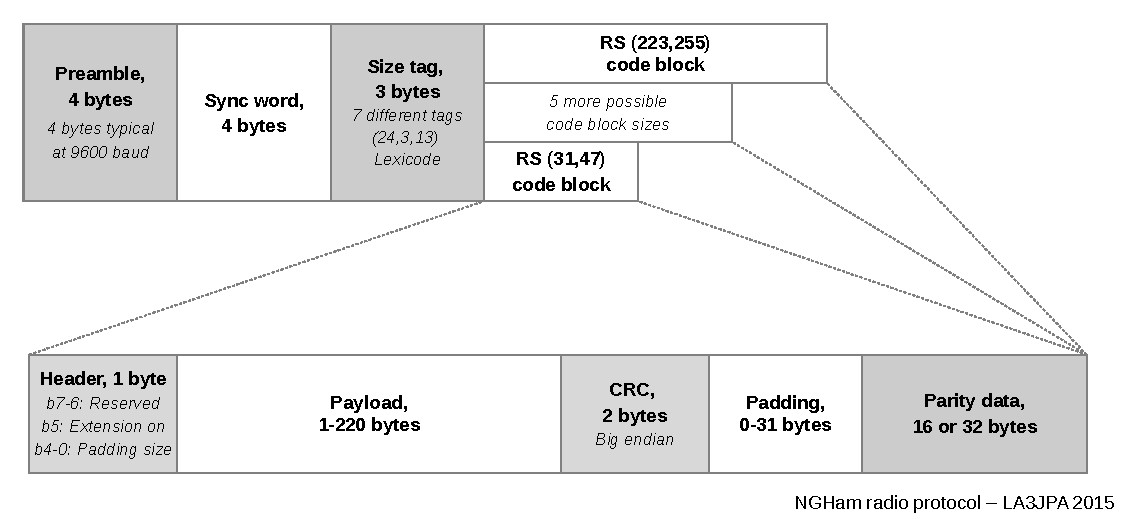
\includegraphics[width=\textwidth]{figures/ngham_block_v4.pdf}
        \caption{NGHam packet structure.}
        \label{fig:ngham-stack}
    \end{center}
\end{figure}

\subsection{CSP}

The CubeSat Space Protocol (CSP) \cite{csp} is a small protocol stack written in C. CSP is designed to ease communication between distributed embedded systems in smaller networks, such as CubeSats. The design follows the TCP/IP model and includes a transport protocol, a routing protocol and several MAC-layer interfaces. The core of libcsp includes a router, a connection oriented socket API and message/connection pools.

The idea is to give sub-system developers of CubeSats the same features of a TCP/IP stack, but without adding the huge overhead of the IP header. The small footprint and simple implementation allows a small 8-bit system to be fully connected on the network. This allows all subsystems to provide their services on the same network level, without any master node required. Using a service oriented architecture has several advantages compared to the traditional mater/slave topology used on many cubesats.

The OBDH's firmware currently uses the version \href{https://github.com/GomSpace/libcsp/releases/tag/1.5.16}{v1.5.16} of the libcsp library.
